\documentclass[]{article}
\usepackage{lmodern}
\usepackage{color}
\usepackage{amssymb,amsmath}
\usepackage{ifxetex,ifluatex}
\usepackage{fixltx2e} % provides \textsubscript
\ifnum 0\ifxetex 1\fi\ifluatex 1\fi=0 % if pdftex
  \usepackage[T1]{fontenc}
  \usepackage[utf8]{inputenc}
\else % if luatex or xelatex
  \ifxetex
    \usepackage{mathspec}
  \else
    \usepackage{fontspec}
  \fi
  \defaultfontfeatures{Ligatures=TeX,Scale=MatchLowercase}
\fi
% use up if available, for straight quotes in verbatim environments
\IfFileExists{upquote.sty}{\usepackage{upquote}}{}
% use microtype if available
\IfFileExists{microtype.sty}{%
\usepackage[]{microtype}
\UseMicrotypeSet[protrusion]{basicmath} % disable protrusion for tt fonts
}{}
\PassOptionsToPackage{hyphens}{url} % url is loaded by hyperref
\usepackage[unicode=true]{hyperref}
\hypersetup{
            pdftitle={arc42 Template},
            pdfborder={0 0 0},
            breaklinks=true}
\urlstyle{same}  % don't use monospace font for urls
\usepackage{longtable,booktabs}
% Fix footnotes in tables (requires footnote package)
\IfFileExists{footnote.sty}{\usepackage{footnote}\makesavenoteenv{long table}}{}
\usepackage{graphicx,grffile}
\makeatletter
\def\maxwidth{\ifdim\Gin@nat@width>\linewidth\linewidth\else\Gin@nat@width\fi}
\def\maxheight{\ifdim\Gin@nat@height>\textheight\textheight\else\Gin@nat@height\fi}
\makeatother
% Scale images if necessary, so that they will not overflow the page
% margins by default, and it is still possible to overwrite the defaults
% using explicit options in \includegraphics[width, height, ...]{}
\setkeys{Gin}{width=\maxwidth,height=\maxheight,keepaspectratio}
\IfFileExists{parskip.sty}{%
\usepackage{parskip}
}{% else
\setlength{\parindent}{0pt}
\setlength{\parskip}{6pt plus 2pt minus 1pt}
}
\setlength{\emergencystretch}{3em}  % prevent overfull lines
\providecommand{\tightlist}{%
  \setlength{\itemsep}{0pt}\setlength{\parskip}{0pt}}
\setcounter{secnumdepth}{0}
% Redefines (sub)paragraphs to behave more like sections
\ifx\paragraph\undefined\else
\let\oldparagraph\paragraph
\renewcommand{\paragraph}[1]{\oldparagraph{#1}\mbox{}}
\fi
\ifx\subparagraph\undefined\else
\let\oldsubparagraph\subparagraph
\renewcommand{\subparagraph}[1]{\oldsubparagraph{#1}\mbox{}}
\fi

% set default figure placement to htbp
\makeatletter
\def\fps@figure{htbp}
\makeatother


\title{
\includegraphics{images/arc42-logo.png} Architektur-Dokumentation zu ShareIt}
\date{2017-06-19}

\begin{document}
\maketitle
\newpage
\section{Einführung und Ziele}\label{section-introduction-and-goals}
Beschreibt die wesentliche Anforderungen und treibenden Kräfte, die
Softwarearchitekten und Entwicklungsteams berücksichtigen müssen. Dazu
gehören die

\begin{itemize}
\item
  zugrunde liegenden Ziele, wesentliche Aufgabenstellung und
  essenzielle fachliche Anforderungen an das System
\item
  Qualitätsziele für die Architektur
\item
  relevante Stakeholder und deren Erwartungshaltung
\end{itemize}

\subsection{Aufgabenstellung}\label{_aufgabenstellung}
\textbf{Inhalt.}

Studierende der Hochschule München benötigen innerhalb der Bachelor-/Master-Laufbahn diverse Fachbücher/CDs um einen intensiven und schnellen Lernerfolg zu erreichen. Diese Literatur ist oftmals kostspielig und wird darüber hinaus meist nur für einen kurzen Zeitraum (für gewöhnlich ein Semester) benötigt. Für diese Problemstellung soll das "ShareIt"-System eine elegante Möglichkeit bieten, um

\begin{itemize}
	\item Studierende nicht mehr benötigte Fachbücher/CDs für den Verleih anzubieten.
	\item benötigte Fachbücher einfach und komfortable ausleihen zu können.
\end{itemize}

Das ShareIt-System soll dabei als zentrale Verleihbibliothek für gebrauchte Fachliteratur/CDs dienen. Studierende, welche Exemplare ausleihen/anbieten wollen, müssen sich gegenüber dem System mittels einem Token authentisieren, um Falscheingaben und Missbrauch zu vermeiden. Die Implementierung wird ohne Front-End zur Verfügung gestellt und nur über eine REST-API implementiert. Als Datenübertragungsformat dient JSON.

Die genaue Anforderungsbeschreibung ist unter Moodle der Veranstaltung "Software-Architektur" verfügbar.

\subsection{Qualitätsziele}\label{_qualit_tsziele}

\textbf{Inhalt.}

Folgende Qualitätsziele sind zwingend erforderlich: 

\begin{itemize}
	\item Hochverfügbarkeit des Systems
	\item Konsistente Datenhaltung
	\item Intuitive und einfache REST-Schnittstelle
\end{itemize}

\colorbox{red} {// evtl. noch Ablauf/Aktivitätsdiagramm hinzufügen}

\textbf{Motivation.}

Mit den Qualitätszielen sollen verschiedene Ziele erreicht werden. Zum einen soll Studenten dauerhaft und zu jeder Tages- und Nachtzeit die Möglichkeit gegeben werden, auf den Service zuzugreifen. Für Abschlussarbeiten ist diese Verfügbarkeit besonders wichtig. (Stichwort Hochverfügbarkeit).

Da Studenten ein Interesse daran haben, ihre Bücher ggf. wieder zurückzufordern, soll auch die Datenhaltung unbedingt konsistent sein. Somit ist garantiert, dass die Eigentümer wissen, wo ihre Bücher zu jedem Zeitpunkt sind. (Stichwort Konsistente Datenhaltung)

Schließlich soll die Schnittstelle möglichst einfach bedienbar sein, sodass ein mögliches Frontend ohne größere Komplikationen darauf aufbauen kann.


\textbf{Form.}

\colorbox{red} {// evtl. noch tabellarische Form hinzufügen}

Tabellarische Darstellung der Qualitätsziele mit möglichst konkreten
Szenarien, geordnet nach Prioritäten.

\subsection{Stakeholder}\label{_stakeholder}

\textbf{Inhalt.}

Stakeholder des Systems sind in erster Linie die Studenten der Hochschule München sowie die Administratoren des Systems. Studenten können dabei als Ausleiher und/oder als Anbieter fungieren, daher wird dessen Funktion in zwei Bereiche aufgeteilt. Folgendes Use Case Diagramm verdeutlicht die Zusammenhänge:

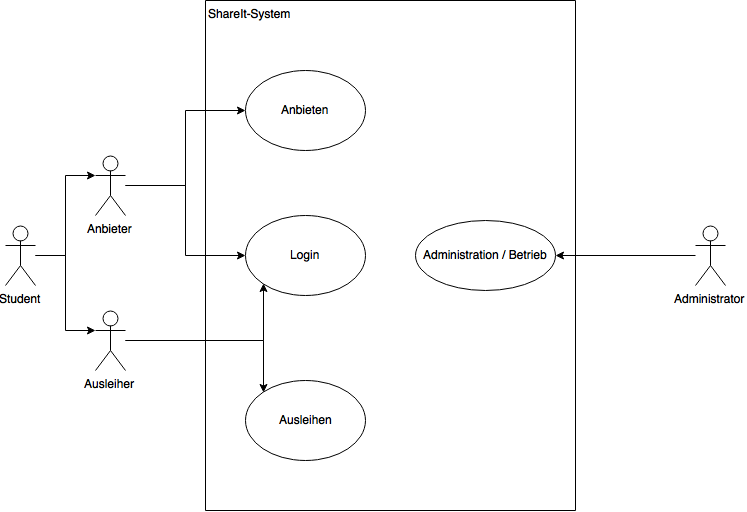
\includegraphics{images/UseCaseDiagram.png}[H]
\begin{itemize}
\item
  die Architektur kennen sollten oder
\item
  von der Architektur überzeugt werden müssen,
\item
  mit Architektur oder Code arbeiten (z.B. Schnittstellen nutzen),
\item
  Dokumentation der Architektur für ihre eigene Arbeit benötigen,
\item
  Entscheidungen über das System und dessen Entwicklung treffen.
\end{itemize}

\textbf{Motivation.}

Für die Administratoren ist die Beschreibung des Systems wichtig, da diese das System entwickeln, betreiben sowie supporten müssen.
Die eigentliche Zielgruppe des Systems ist an die Studenten der Hochschule München gerichtet, welche somit Hauptbestandteil des Systems sind und zwingend als Stakeholder aufgenommen werden müssen.

\textbf{Form.}

Tabelle mit Rollen- oder Personennamen, sowie deren Erwartungshaltung
bezüglich der Architektur und deren Dokumentation.


\section{Randbedingungen}\label{section-architecture-constraints}

Wichtige Randbedingung ist z.B., dass eine sichere Authentifizierung am System erfolgen muss. Des Weiteren muss eine klar erkennbare Schichtenarchitektur befolgt werden, sodass keine unerlaubten Abhängigkeiten innerhalb der REST-Architektur bestehen.

Grundsätzlich sollen die Bestandteile des Systems als gesamtes als OpenSource-Projekt zur Vefügung stehen. Die Implementierung soll in der Programmiersprache Java erfolgen. Eingebettet in einen Jetty-Server soll das Jersey RESTful-Webservices Framework anhand der JAX-RS Bibliothek zur Implementierung verwendet werden. 
Für die Persistenzierung ist Hibernate vorgesehen.

Organisatorisch: Das Entwicklerteam soll aus mindestens zwei und höchstens vier Entwickler(inne)n zusammengesetzt sein.

\textbf{Inhalt.}

Fesseln und Vorgaben, die ihre Freiheiten bezüglich Entwurf,
Implementierung oder Ihres Entwicklungsprozesses einschränken. Diese
Randbedingungen gelten manchmal organisations- oder firmenweit über die
Grenzen einzelner Systeme hinweg.

\textbf{Motivation.}

Als Architekt sollten Sie explizit wissen, wo Ihre Freiheitsgrade
bezüglich Entwurfsentscheidungen liegen und wo Sie Randbedingungen
beachten müssen. Sie können Randbedingungen vielleicht noch verhandeln,
zunächst sind sie aber da.

\textbf{Form.}

Einfache Tabellen der Randbedingungen mit Erläuterungen. Bei Bedarf
unterscheiden Sie technische, organisatorische und politische
Randbedingungen oder übergreifende Konventionen (beispielsweise
Programmier- oder Versionierungsrichtlinien, Dokumentation- oder
Namenskonvention)

\section{Kontextabgrenzung}\label{section-system-scope-and-context}

\colorbox{red} {// REST-Schnittstellenbeschreibung hinzufügen, z.B. swagger}
\textbf{Inhalt.}

Die Kontextabgrenzung grenzt das System von allen Kommunikationspartnern
(Nachbarsystemen und Benutzerrollen) ab. Sie legt damit die externen
Schnittstellen fest.

Differenzieren Sie fachlichen Kontext (fachliche Ein- und Ausgaben) und
technischen Kontext (Kanäle, Protokolle, Hardware), falls nötig.

\textbf{Motivation.}

Die fachlichen und technischen Schnittstellen zu Kommunikationspartnern
gehören zu den kritischsten Aspekten eines Systems. Stellen Sie sicher,
dass Sie diese komplett verstanden haben.

\textbf{Form.}

Verschiedene Optionen:

\begin{itemize}
\item
  Diverse Kontextdiagramme
\item
  Listen von Kommunikationspartnern mit deren Schnittstellen
\end{itemize}

\subsection{Fachlicher Kontext}\label{_fachlicher_kontext}

\textbf{Inhalt.}

Festlegung \textbf{aller} Kommunikationspartner (Nutzer, IT-Systeme,
\ldots{}) mit Erklärung der fachlichen Ein- und Ausgabedaten oder
Schnittstellen. Zusätzlich bei Bedarf fachliche Datenformate oder
Protokolle der Kommunikation mit den Nachbarsystemen.

\textbf{Motivation.}

Alle Beteiligten müssen verstehen, welche fachlichen Informationen mit
der Umwelt ausgetauscht werden.

\textbf{Form.}

Alle Diagrammarten, die das System als Black Box darstellen und die
fachlichen Schnittstellen zu den Nachbarn beschreiben.

Alternativ oder ergänzend können Sie eine Tabelle verwenden. Der Titel
gibt den Namen Ihres Systems wieder; die drei Spalten sind:
Kommunikationspartner, Eingabe, Ausgabe.

\textbf{\textless{}Diagramm und/oder Tabelle\textgreater{}}

\textbf{\textless{}optional: Erläuterung der externen fachlichen
Schnittstellen\textgreater{}}

\subsection{Technischer Kontext}\label{_technischer_kontext}

\textbf{Inhalt.}

Technische Schnittstellen (Kanäle, Übertragungsmedien) zwischen dem
System und seiner Umwelt. Zusätzlich eine Erklärung (\emph{mapping}),
welche fachlichen Ein- und Ausgaben über welche technischen Kanäle
fließen.

\textbf{Motivation.}

Viele Stakeholder treffen Architekturentscheidungen auf Basis der
technischen Schnittstellen des Systems zu seinem Kontext.

Insbesondere Infrastruktur- oder Hardwareentwickler entscheiden auch
über diese technischen Schnittstellen.

\textbf{Form.}

Beispielsweise UML Deployment-Diagramme mit den Kanälen zu
Nachbarsystemen, begleitet von einer Tabelle, die Kanäle auf
Ein-/Ausgaben abbildet.

\textbf{\textless{}Diagramm oder Tabelle\textgreater{}}

\textbf{\textless{}optional: Erläuterung der externen technischen
Schnittstellen\textgreater{}}

\textbf{\textless{}Mapping fachliche auf technische
Schnittstellen\textgreater{}}

\section{Lösungsstrategie}\label{section-solution-strategy}

Es wird bewusst auf eine Lösung mittels eines REST-Services gesetzt, da somit bereits das Grundgerüst der Infrastruktur für einen Webservice vorhanden ist.

Die Schichtenarchitektur hilft dabei, eine möglichst klare Struktur zu schaffen und z.B. einzelne Schichten getrennt voneinander betrachten/austauschen zu können. Somit wird nicht nur dem Nutzer, sondern auch den Administratoren das Leben erleichtert.

Qualitätstechnisch wird so z.B. erreicht, dass eine einfache und intuitive REST-Schnittstelle zur Vefügung gestellt werden kann. Außerdem wird das Ziel der konsistenten Datenhaltung maßgeblich unterstützt, da das Risiko von Inkonsistenzen in der Datenhaltungsschicht durch die strikte Schichtenarchitektur minimiert werden kann.

\textbf{Inhalt.}

Kurzer Überblick über die grundlegenden Entscheidungen und
Lösungsansätze, die Entwurf und Implementierung des Systems prägen.
Hierzu gehören:

\begin{itemize}
\item
  Technologieentscheidungen
\item
  Entscheidungen über die Top-Level-Zerlegung des Systems,
  beispielsweise die Verwendung gesamthaft prägender Entwurfs- oder
  Architekturmuster
\item
  Entscheidungen zur Erreichung der wichtigsten Qualitätsanforderungen
\item
  relevante organisatorische Entscheidungen, beispielsweise für
  bestimmte Entwicklungsprozesse oder Delegation bestimmter Aufgaben an
  andere Stakeholder.
\end{itemize}

\textbf{Motivation.}

Diese allerwichtigsten Entscheidungen bilden wesentliche „Eckpfeiler``
der Architektur. Von ihnen hängen meistens viele weitere Entscheidungen
oder Implementierungsregeln ab.

\textbf{Form.}

Fassen Sie die zentralen Entwurfsentscheidungen \textbf{kurz} zusammen.
Motivieren Sie ausgehend von Aufgabenstellung, Qualitätszielen und
Randbedingungen, was Sie entschieden haben und warum Sie so entschieden
haben. Verweisen Sie eher auf weitere Ausführungen in Folgeabschnitten.

\section{Bausteinsicht}\label{section-building-block-view}
Die Architektur der Software ist wie folgt in Schichtenmodell aufgebaut:
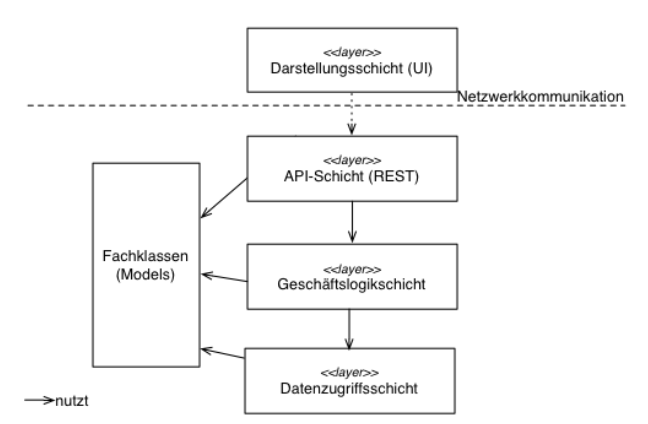
\includegraphics{images/SoftwareLayers.png}

Dabei dient die "Resourcen"-Schicht als oberste Layer, welche alle Schnittstellen der REST-API implementieren und ggfs. JSON in Objekte umwandeln bzw. im Falle einer Antwort Objekte zurück in JSON umwandelt. Die Ressourcen-Schicht beinhaltet dabei keinerlei Überprüfung der ankommenden Daten. Die Prüfung auf fehlerhafte bzw. unvollständige Daten wird in der Geschäftslogikschicht durchgeführt, welche von der REST-API-Schicht an die Geschäftslogikschicht gesendet wird. Diese prüft die eingehenden Daten und definiert, ob Daten gespeichert werden und welche Antwort (Response) an den Client zurückgesendet wird. Dabei kommuniziert die Geschäftslogikschicht nicht direkt mit der Datenbank, sondern leitet diese Anfragen an die Datenzugrifsschicht weiter. Diese enthält Informationen zur Datenbankanbidung und stellt enstsprechende Methoden für die Geschäftslogikschicht für Abfragen (inserts, update, exists, etc.) Verfügung.

Neben den Schichten werden sog. Fachklassen (Models) bereitgestellt, welche schichtenübergreifend Objekte für die Modellierung von Books, Discs, Mediums, Tokens und Users zur Verfügung stellt. Diese beinhalten keinerlei Logik und werden nur als Objekte verwendet, welche zu realen, abstrahierten Informationen zugeordnet werden.

Hinweis: Die Darstellungsschicht (UI) ist nicht Bestandteil des ShareIt-Systems und muss vom Nutzer der REST-API selbst implementiert werden. (sofern benötigt)

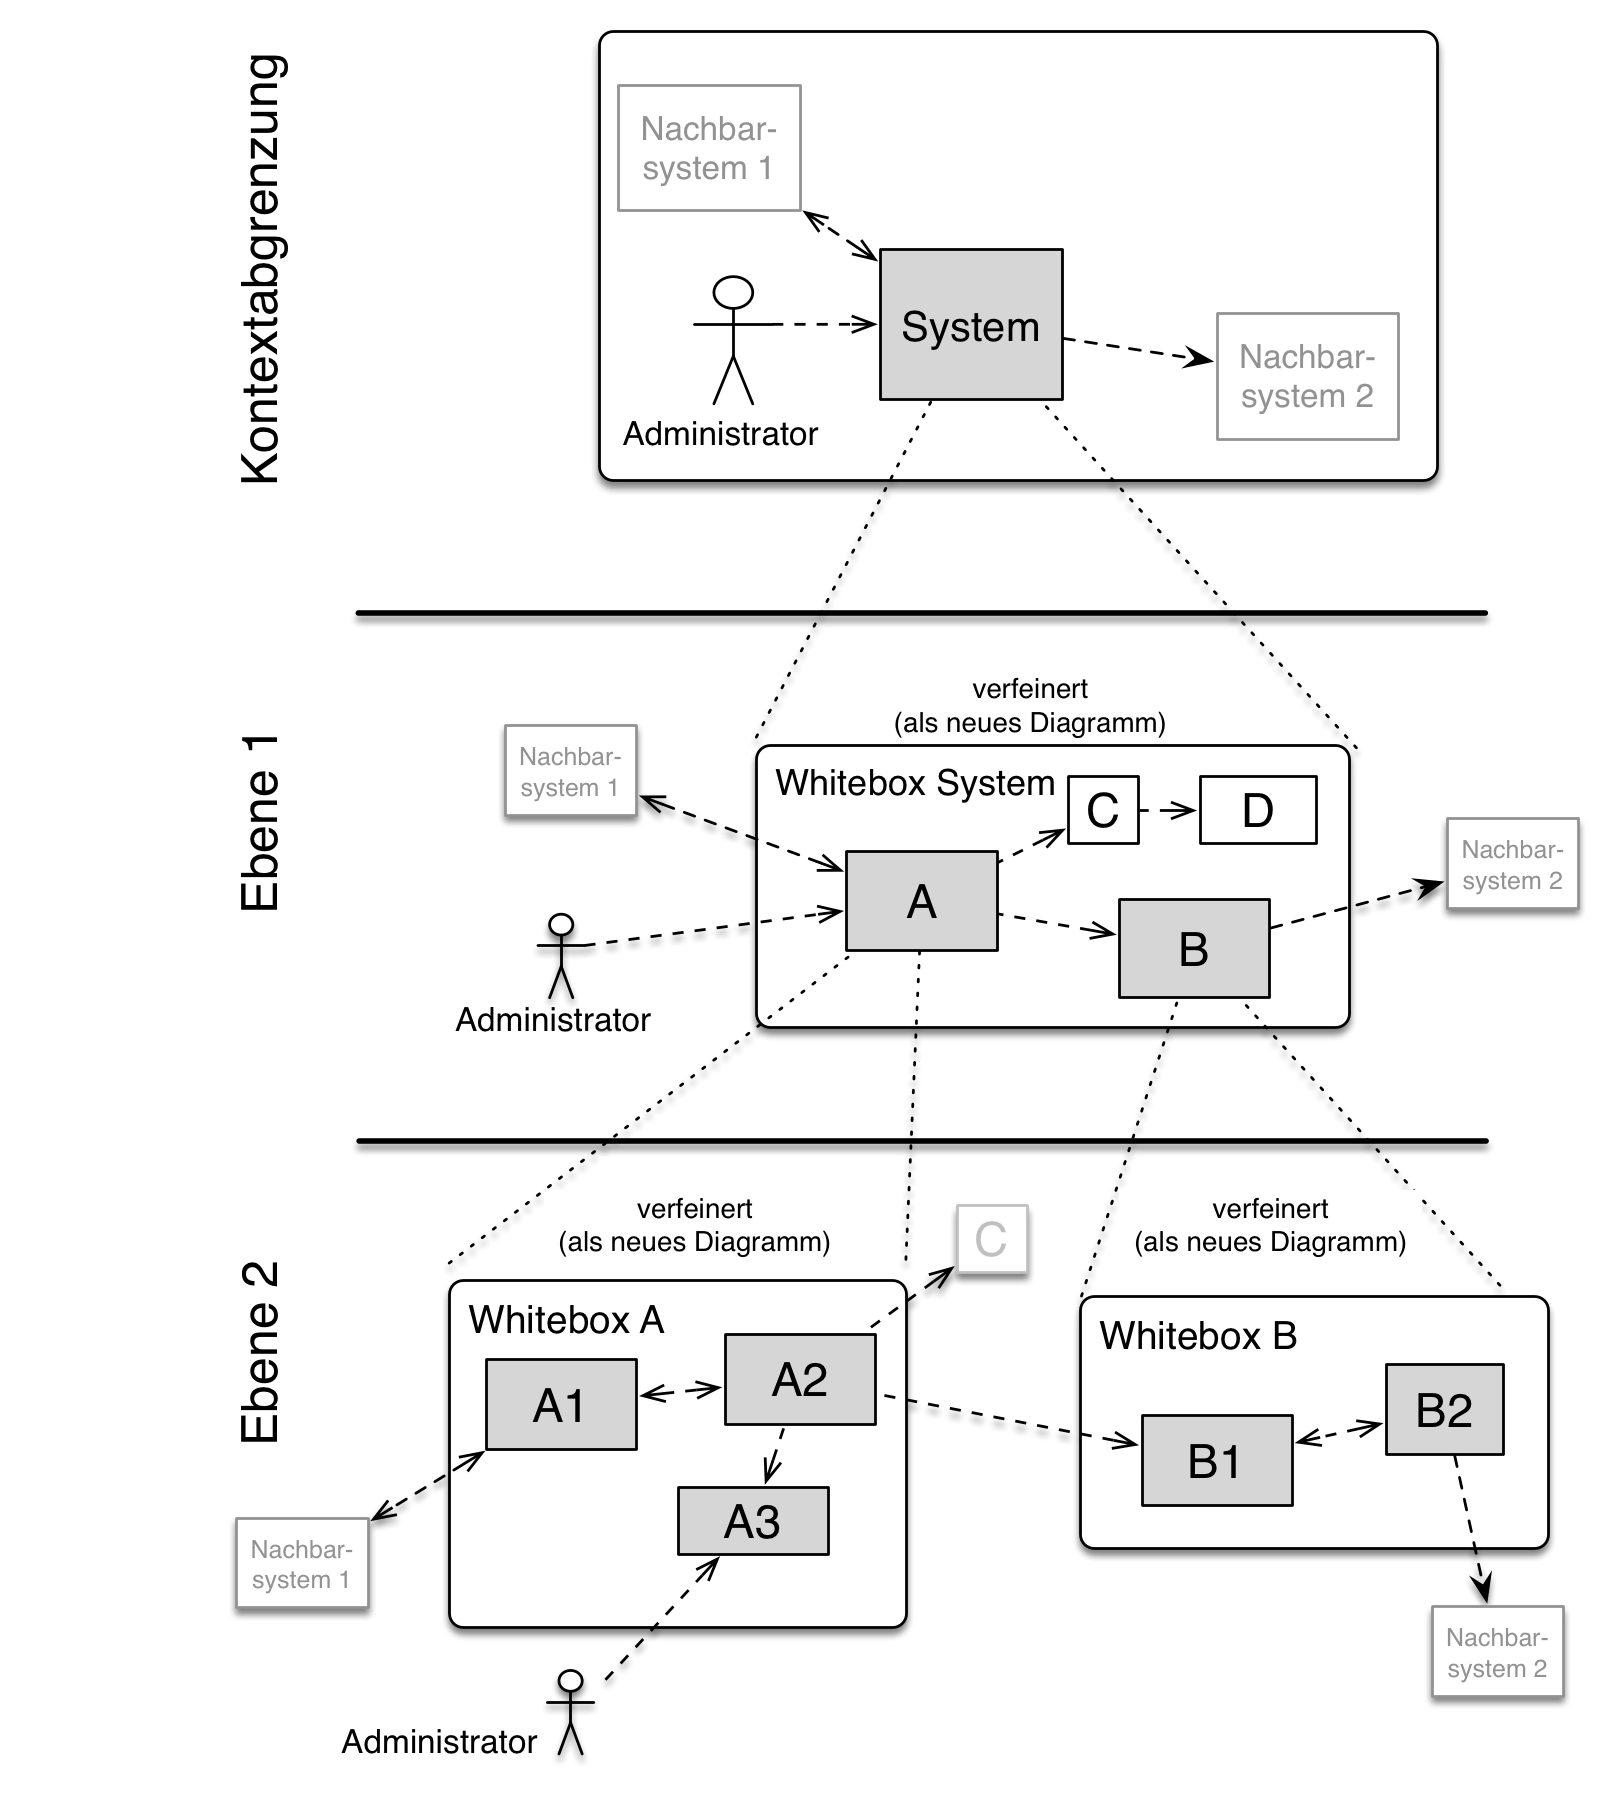
\includegraphics{images/05_building_blocks-DE.png}

\subsection{Whitebox Gesamtsystem}\label{_whitebox_gesamtsystem}

An dieser Stelle beschreiben Sie die Zerlegung des Gesamtsystems anhand
des nachfolgenden Whitebox-Templates. Dieses enthält:

\begin{itemize}
\item
  Ein Übersichtsdiagramm
\item
  die Begründung dieser Zerlegung
\item
  Blackbox-Beschreibungen der hier enthaltenen Bausteine. Dafür haben
  Sie verschiedene Optionen:

  \begin{itemize}
  \item
    in \emph{einer} Tabelle, gibt einen kurzen und pragmatischen
    Überblick über die enthaltenen Bausteine sowie deren Schnittstellen.
  \item
    als Liste von Blackbox-Beschreibungen der Bausteine, gemäß dem
    Blackbox-Template (siehe unten). Diese Liste können Sie, je nach
    Werkzeug, etwa in Form von Unterkapiteln (Text), Unter-Seiten (Wiki)
    oder geschachtelten Elementen (Modellierungswerkzeug) darstellen.
  \end{itemize}
\item
  (optional:) wichtige Schnittstellen, die nicht bereits im
  Blackbox-Templates eines der Bausteine erläutert werden, aber für das
  Verständnis der Whitebox von zentraler Bedeutung sind. Aufgrund der
  vielfältigen Möglichkeiten oder Ausprägungen von Schnittstellen geben
  wir hierzu kein weiteres Template vor. Im schlimmsten Fall müssen Sie
  Syntax, Semantik, Protokolle, Fehlerverhalten, Restriktionen,
  Versionen, Qualitätseigenschaften, notwendige Kompatibilitäten und
  vieles mehr spezifizieren oder beschreiben. Im besten Fall kommen Sie
  mit Beispielen oder einfachen Signaturen zurecht.
\end{itemize}

\emph{\textbf{\textless{}Übersichtsdiagramm\textgreater{}}}

\begin{description}
\item[Begründung]
\emph{\textless{}Erläuternder Text\textgreater{}}
\item[Enthaltene Bausteine]
\emph{\textless{}Beschreibung der enhaltenen Bausteine
(Blackboxen)\textgreater{}}
\item[Wichtige Schnittstellen]
\emph{\textless{}Beschreibung wichtiger Schnittstellen\textgreater{}}
\end{description}

Hier folgen jetzt Erläuterungen zu Blackboxen der Ebene 1.

Falls Sie die tabellarische Beschreibung wählen, so werden Blackboxen
darin nur mit Name und Verantwortung nach folgendem Muster beschrieben:

\begin{longtable}[]{@{}ll@{}}
\toprule
\begin{minipage}[b]{0.31\columnwidth}\raggedright\strut
\textbf{Name}\strut
\end{minipage} & \begin{minipage}[b]{0.63\columnwidth}\raggedright\strut
\textbf{Verantwortung}\strut
\end{minipage}\tabularnewline
\midrule
\endhead
\begin{minipage}[t]{0.31\columnwidth}\raggedright\strut
\emph{\textless{}Blackbox 1\textgreater{}}\strut
\end{minipage} & \begin{minipage}[t]{0.63\columnwidth}\raggedright\strut
~\emph{\textless{}Text\textgreater{}}\strut
\end{minipage}\tabularnewline
\begin{minipage}[t]{0.31\columnwidth}\raggedright\strut
\emph{\textless{}Blackbox 2\textgreater{}}\strut
\end{minipage} & \begin{minipage}[t]{0.63\columnwidth}\raggedright\strut
~\emph{\textless{}Text\textgreater{}}\strut
\end{minipage}\tabularnewline
\bottomrule
\end{longtable}

Falls Sie die ausführliche Liste von Blackbox-Beschreibungen wählen,
beschreiben Sie jede wichtige Blackbox in einem eigenen
Blackbox-Template. Dessen Überschrift ist jeweils der Namen dieser
Blackbox.

\subsubsection{\textless{}Name Blackbox
1\textgreater{}}\label{__name_blackbox_1}

An dieser Stelle beschreiben Sie die \textless{}Blackbox 1\textgreater{}
anhand des folgenden Blackbox-Templates:

\begin{itemize}
\item
  Zweck/Verantwortung
\item
  Schnittstelle(n), sofern sie nicht als eigenständige Beschreibungen
  herausgezogen sind. Hierzu gehören eventuell auch Qualitäts- und
  Leistungsmerkmale dieser Schnittstelle.
\item
  (Optional) Qualitäts-/Leistungsmerkmale der Blackbox, beispielsweise
  Verfügbarkeit, Laufzeitverhalten\ldots{}
\item
  (Optional) Ablageort/Datei(en)
\item
  (Optional) Erfüllte Anforderungen, falls Sie Traceability zu
  Anforderungen benötigen.
\item
  (Optional) Offene Punkte/Probleme/Risiken
\end{itemize}

\emph{\textless{}Zweck/Verantwortung\textgreater{}}

\emph{\textless{}Schnittstelle(n)\textgreater{}}

\emph{\textless{}(Optional) Qualitäts-/Leistungsmerkmale\textgreater{}}

\emph{\textless{}(Optional) Ablageort/Datei(en)\textgreater{}}

\emph{\textless{}(Optional) Erfüllte Anforderungen\textgreater{}}

\emph{\textless{}(optional) Offene
Punkte/Probleme/Risiken\textgreater{}}

\subsubsection{\textless{}Name Blackbox
2\textgreater{}}\label{__name_blackbox_2}

\emph{\textless{}Blackbox-Template\textgreater{}}

\subsubsection{\textless{}Name Blackbox
n\textgreater{}}\label{__name_blackbox_n}

\emph{\textless{}Blackbox-Template\textgreater{}}

\subsubsection{\textless{}Name Schnittstelle
1\textgreater{}}\label{__name_schnittstelle_1}

\ldots{}

\subsubsection{\textless{}Name Schnittstelle
m\textgreater{}}\label{__name_schnittstelle_m}

\subsection{Ebene 2}\label{_ebene_2}

An dieser Stelle können Sie den inneren Aufbau (einiger) Bausteine aus
Ebene 1 als Whitebox beschreiben.

Welche Bausteine Ihres Systems Sie hier beschreiben, müssen Sie selbst
entscheiden. Bitte stellen Sie dabei Relevanz vor Vollständigkeit.
Skizzieren Sie wichtige, überraschende, riskante, komplexe oder
besonders volatile Bausteine. Normale, einfache oder standardisierte
Teile sollten Sie weglassen.

\subsubsection{\texorpdfstring{Whitebox \emph{\textless{}Baustein
1\textgreater{}}}{Whitebox \textless{}Baustein 1\textgreater{}}}\label{_whitebox_emphasis_baustein_1_emphasis}

\ldots{}zeigt das Innenleben von \emph{Baustein 1}.

\emph{\textless{}Whitebox-Template\textgreater{}}

\subsubsection{\texorpdfstring{Whitebox \emph{\textless{}Baustein
2\textgreater{}}}{Whitebox \textless{}Baustein 2\textgreater{}}}\label{_whitebox_emphasis_baustein_2_emphasis}

\emph{\textless{}Whitebox-Template\textgreater{}}

\ldots{}

\subsubsection{\texorpdfstring{Whitebox \emph{\textless{}Baustein
m\textgreater{}}}{Whitebox \textless{}Baustein m\textgreater{}}}\label{_whitebox_emphasis_baustein_m_emphasis}

\emph{\textless{}Whitebox-Template\textgreater{}}

\subsection{Ebene 3}\label{_ebene_3}

An dieser Stelle können Sie den inneren Aufbau (einiger) Bausteine aus
Ebene 2 als Whitebox beschreiben.

Bei tieferen Gliederungen der Architektur kopieren Sie diesen Teil von
arc42 für die weiteren Ebenen.

\subsubsection{Whitebox \textless{}\_Baustein
x.1\_\textgreater{}}\label{_whitebox_baustein_x_1}

\ldots{}zeigt das Innenleben von \emph{Baustein x.1}.

\emph{\textless{}Whitebox-Template\textgreater{}}

\subsubsection{Whitebox \textless{}\_Baustein
x.2\_\textgreater{}}\label{_whitebox_baustein_x_2}

\emph{\textless{}Whitebox-Template\textgreater{}}

\subsubsection{Whitebox \textless{}\_Baustein
y.1\_\textgreater{}}\label{_whitebox_baustein_y_1}

\emph{\textless{}Whitebox-Template\textgreater{}}

\section{Laufzeitsicht}\label{section-runtime-view}

\textbf{Inhalt.}

Diese Sicht erklärt konkrete Abläufe und Beziehungen zwischen Bausteinen
in Form von Szenarien aus folgenden Bereichen:

\begin{itemize}
\item
  Wichtige Abläufe oder \emph{Features}: Wie führen die Bausteine der
  Architektur die wichtigsten Abläufe durch?
\item
  Interaktionen an kritischen externen Schnittstellen: Wie arbeiten
  Bausteine mit Nutzern und Nachbarsystemen zusammen?
\item
  Betrieb und Administration: Inbetriebnahme, Start, Stop.
\item
  Fehler- und Ausnahmeszenarien
\end{itemize}

Anmerkung: Kriterium für die Auswahl der möglichen Szenarien (d.h.
Abläufe) des Systems ist deren Architekturrelevanz. Es geht nicht darum,
möglichst viele Abläufe darzustellen, sondern eine angemessene Auswahl
zu dokumentieren.

\textbf{Motivation.}

Sie sollten verstehen wie (Instanzen von) Bausteine(n) Ihres Systems
ihre jeweiligen Aufgaben erfüllen und zur Laufzeit miteinander
kommunizieren.

Nutzen Sie solche Szenarien in der Dokumentation hauptsächlich zur
besseren Kommunikation mit Stakeholdern, die statische Modelle (z.B.
Bausteinsicht, Verteilungssicht) weniger verständlich finden.

\textbf{Form.}

Für die Beschreibung von Szenarien gibt es zahlreiche
Ausdrucksmöglichkeiten. Nutzen Sie beispielsweise:

\begin{itemize}
\item
  Nummerierte Schrittfolgen oder Aufzählungen in Umgangssprache
\item
  Aktivitäts- oder Flussdiagramme
\item
  Sequenzdiagramme
\item
  BPMN oder EPKs (Ereignis-Prozessketten)
\item
  Zustandsautomaten
\item
  \ldots{}
\end{itemize}

\subsection{\texorpdfstring{\emph{\textless{}Bezeichnung
Laufzeitszenario
1\textgreater{}}}{\textless{}Bezeichnung Laufzeitszenario 1\textgreater{}}}\label{__emphasis_bezeichnung_laufzeitszenario_1_emphasis}

\begin{itemize}
\item
  \textless{}hier Laufzeitdiagramm oder Ablaufbeschreibung
  einfügen\textgreater{}
\item
  \textless{}hier Besonderheiten bei dem Zusammenspiel der Bausteine in
  diesem Szenario erläutern\textgreater{}
\end{itemize}

\subsection{\texorpdfstring{\emph{\textless{}Bezeichnung
Laufzeitszenario
2\textgreater{}}}{\textless{}Bezeichnung Laufzeitszenario 2\textgreater{}}}\label{__emphasis_bezeichnung_laufzeitszenario_2_emphasis}

\ldots{}

\subsection{\texorpdfstring{\emph{\textless{}Bezeichnung
Laufzeitszenario
n\textgreater{}}}{\textless{}Bezeichnung Laufzeitszenario n\textgreater{}}}\label{__emphasis_bezeichnung_laufzeitszenario_n_emphasis}

\ldots{}

\section{Verteilungssicht}\label{section-deployment-view}

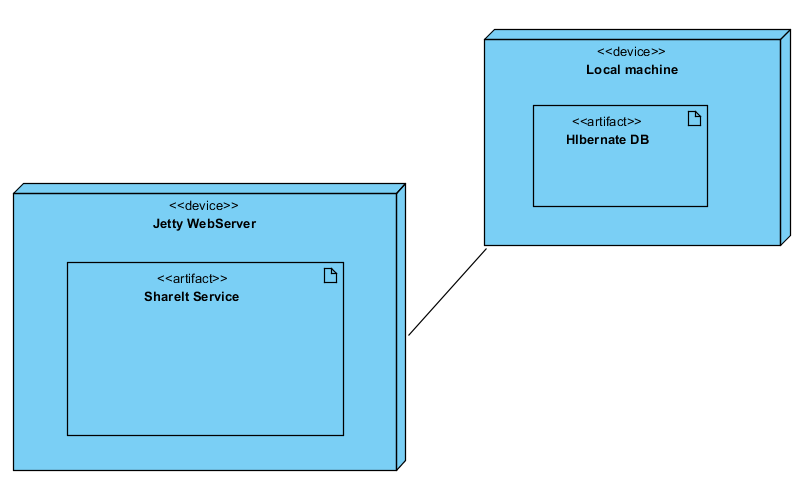
\includegraphics{images/UMLDeploymentDiag.PNG}

Die Infrastruktur des ShareIt Systems ist recht übersichtlich, innerhalb des Jetty WebServers wird der ShareIt Service (inkl. Authentifizierungsservice) ausgeführt, während die Hibernate Datenbank auf der jeweiligen lokalen Maschine ausgeführt wird.



\section{Querschnittliche Konzepte}\label{section-concepts}



\textbf{Fachliches Datenmodell}

Das fachliche Datenmodell beinhaltet die Entitäten, die für das System relevant sind, in diesem Fall Books und Discs (leiten beide von Medium ab), Copies sowie Token und User. Die jeweilige Funktion der einzelnen Entitäten ist mittels JavaDoc genau beschrieben.

\textbf{Logging}

Im gesamten System wird ein Logging-Tool verwendet (log4j), das dabei hilft, den Programmcode zur Runtime verständlicher und besser nachvollziehbar zu machen. log4j wird dabei in den jeweiligen Klassen über einen statischen "LogManager" initialisiert, der dann für die Ausgabe von Informationen, Fehlern, etc... verwendet werden kann.


\textbf{Sicherheit/Session Management}

Um beim Zugriff auf die verschiedenen Schnittstellen der REST-Api die Sicherheit der Daten zu gewährleisten, wurde eine querschnittliche Authentifizierung implementiert. Jeder Nutzer muss sich zunächst einloggen, wodurch er in den darauffolgenden Aktionen eindeutig identifiziert werden kann. Der unter "Fachliches Datenmodell" genannte Token wird hier einmalig generiert und dient beim Zugriff auf die Ressourcen der zuverlässigen Authorisierung.



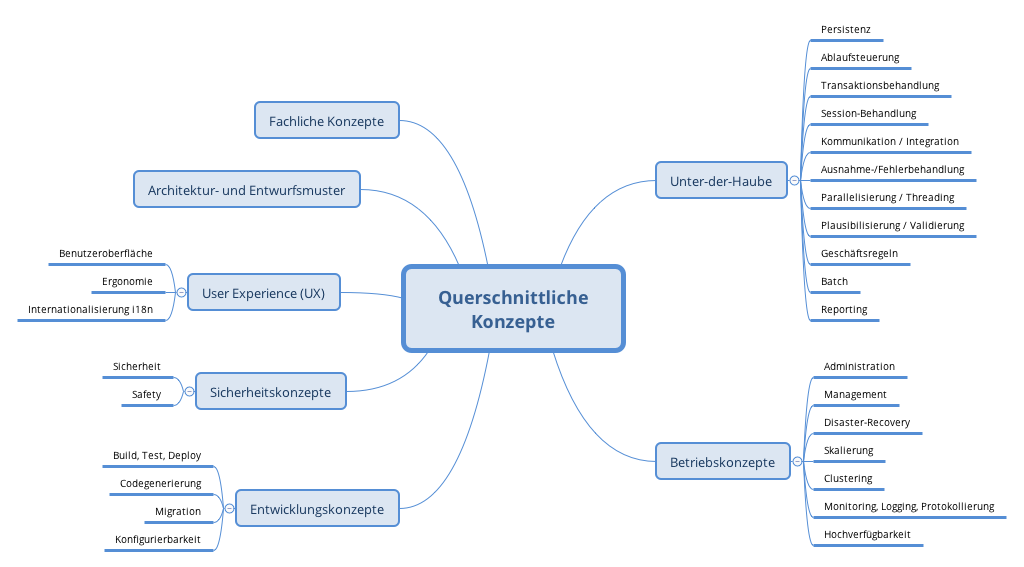
\includegraphics{images/08-Crosscutting-Concepts-Structure-DE.png}


\section{Entwurfsentscheidungen}\label{section-design-decisions}

Wie unter dem Punkt Lösungsstrategie bereits beschrieben, ging es bei den Entwurfsentscheidungen vor allem um die Architektur des WebServices, der den Shareit-Service bereitstellen soll.

Hier standen zunächst die Alternative REST und SOAP zur Verfügung, aufgrund der höheren Flexibilität von REST (z.B. JSON und XML verfügbar), wurde letztlich REST ausgewählt.




\section{Qualitätsanforderungen}\label{section-quality-scenarios}

\textbf{Inhalt.}

Dieser Abschnitt enthält möglichst alle Qualitätsanforderungen als
Qualitätsbaum mit Szenarien. Die wichtigsten davon haben Sie bereits in
Abschnitt 1.2 (Qualitätsziele) hervorgehoben.

Nehmen Sie hier auch Qualitätsanforderungen geringerer Priorität auf,
deren Nichteinhaltung oder -erreichung geringe Risiken birgt.

\textbf{Motivation.}

Weil Qualitätsanforderungen die Architekturentscheidungen oft maßgeblich
beeinflussen, sollten Sie die für Ihre Stakeholder relevanten
Qualitätsanforderungen kennen, möglichst konkret und operationalisiert.

\subsection{Qualitätsbaum}\label{_qualit_tsbaum}

\textbf{Inhalt.}

Der Qualitätsbaum ( a la ATAM) mit Qualitätsszenarien an den Blättern.

\textbf{Motivation.}

Die mit Prioritäten versehene Baumstruktur gibt Überblick über die
oftmals zahlreichen Qualitätsanforderungen.

\begin{itemize}
\item
  Baumartige Verfeinerung des Begriffes „Qualität``, mit "Qualität" oder
  Nützlichkeit als Wurzel.
\item
  Mindmap mit Q-Oberbegriffen als Hauptzweige
\end{itemize}

In jedem Fall sollten Sie hier Verweise auf die Szenarien des folgenden
Abschnittes aufnehmen.

\subsection{Qualitätsszenarien}\label{_qualit_tsszenarien}

\textbf{Inhalt.}

Konkretisierung der (in der Praxis oftmals vagen oder impliziten)
Qualitätsanforderungen durch (Qualitäts-)Szenarien.

Diese Szenarien beschreiben, was beim Eintreffen eines Stimulus auf ein
System in bestimmten Situationen geschieht.

Wesentlich für die meisten Softwarearchitekten sind zwei Arten von
Szenarien:

\begin{itemize}
\item
  Nutzungsszenarien (auch genannt Anwendungs- oder
  Anwendungsfallszenarien) beschreiben, wie das System zur Laufzeit auf
  einen bestimmten Auslöser reagieren soll. Hierunter fallen auch
  Szenarien zur Beschreibung von Effizienz oder Performance. Beispiel:
  Das System beantwortet eine Benutzeranfrage innerhalb einer Sekunde.
\item
  Änderungsszenarien beschreiben eine Modifikation des Systems oder
  seiner unmittelbarer Umgebung. Beispiel: Eine zusätzliche
  Funktionalität wird implementiert oder die Anforderung an ein
  Qualitätsmerkmal ändert sich.
\end{itemize}

\textbf{Motivation.}

Szenarien operationalisieren Qualitätsanforderungen und machen deren
Erfüllung mess- oder entscheidbar.

Insbesondere wenn Sie die Qualität Ihrer Architektur mit Methoden wie
ATAM überprüfen wollen, bedürfen die in Abschnitt 1.2 genannten
Qualitätsziele einer weiteren Präzisierung bis auf die Ebene von
diskutierbaren und nachprüfbaren Szenarien.

\textbf{Form.}

Entweder tabellarisch oder als Freitext.

\section{Risiken und technische Schulden}\label{section-technical-risks}

\textbf{Inhalt.}

Eine nach Prioritäten geordnete Liste der erkannten Architekturrisiken
und/oder technischen Schulden.

\textbf{Motivation.}

"Risikomanagement ist Projektmanagement für Erwachsene" (Tim Lister,
Atlantic Systems Guild.)

Unter diesem Motto sollten Sie Architekturrisiken und/oder technische
Schulden gezielt ermitteln, bewerten und Ihren Management-Stakeholdern
(z.B. Projektleitung, Product-Owner) transparent machen.

\textbf{Form.}

Liste oder Tabelle von Risiko und/oder technischen Schulden, eventuell
mit vorgeschlagenen Maßnahmen zur Risikovermeidung, Risikominimierung
oder dem Abbau der technischen Schulden.

\section{Glossar}\label{section-glossary}

\textbf{Inhalt.}

Die wesentlichen fachlichen und technischen Begriffe, die Stakeholder im
Zusammenhang mit dem System verwenden.

Nutzen Sie das Glossar ebenfalls als Übersetzungsreferenz, falls Sie in
mehrsprachigen Teams arbeiten.

\textbf{Motivation.}

Sie sollten relevante Begriffe klar definieren, so dass alle Beteiligten

\begin{enumerate}
\def\labelenumi{\arabic{enumi}.}
\item
  diese Begriffe identisch verstehen, und
\item
  vermeiden, mehrere Begriffe für die gleiche Sache zu haben.
\end{enumerate}

\begin{itemize}
\item
  Zweispaltige Tabelle mit \textless{}Begriff\textgreater{} und
  \textless{}Definition\textgreater{}
\item
  Eventuell weitere Spalten mit Übersetzungen, falls notwendig.
\end{itemize}

\begin{longtable}[]{@{}ll@{}}
\toprule
\begin{minipage}[b]{0.31\columnwidth}\raggedright\strut
Begriff\strut
\end{minipage} & \begin{minipage}[b]{0.63\columnwidth}\raggedright\strut
Definition\strut
\end{minipage}\tabularnewline
\midrule
\endhead
\begin{minipage}[t]{0.31\columnwidth}\raggedright\strut
\emph{\textless{}Begriff-1\textgreater{}}\strut
\end{minipage} & \begin{minipage}[t]{0.63\columnwidth}\raggedright\strut
\emph{\textless{}Definition-1\textgreater{}}\strut
\end{minipage}\tabularnewline
\begin{minipage}[t]{0.31\columnwidth}\raggedright\strut
\emph{\textless{}Begriff-2}\strut
\end{minipage} & \begin{minipage}[t]{0.63\columnwidth}\raggedright\strut
\emph{\textless{}Definition-2\textgreater{}}\strut
\end{minipage}\tabularnewline
\bottomrule
\end{longtable}

\end{document}
